%This is my Galvanize capstone project presintation

\documentclass{beamer}

%Setting up theme
\usetheme{Frankfurt}
%\usecolortheme{seahorse}
%\usecolortheme{rose}
%\usefonttheme[onlylarge]{structuresmallcapsserif}
%\usefonttheme[onlysmall]{structurebold}

\title{Smart Battery for Smart Energy Usage}
\author{Anatoly Pavlov}
\date{October 20, 2016}

\begin{document}

\begin{frame}
\titlepage
\centering
{Galvanize, San Francisco, Cohort 16}
\end{frame}

\section{Data Science for Smart Grid}
%1
\begin{frame}
\frametitle{Data Science for Smart Grid}
The Smart Grid is the system that always tries to satisfy the equilibrium between energy supply and demand. How does it do it?

\begin{itemize}
\item By utilizing electronic devises (smart meters) which collect data about energy consumption
\item Analysis of obtained data and use of machine learning techniques to derive predictions on energy demand
\item Introduction of energy storage devices (batteries) in households brings new opportunities for a more efficient and reliable energy demand and generation.
\end{itemize}
\end{frame}

\section{Data}
%2
\begin{frame}
\frametitle{London Household Smart Meter Readings}
I used large collection of smart meter data obtained by UK Power Networks a sample of 5,567 London households between November 2011 and February 2014.

\begin{figure}[htb]
\begin{center}
    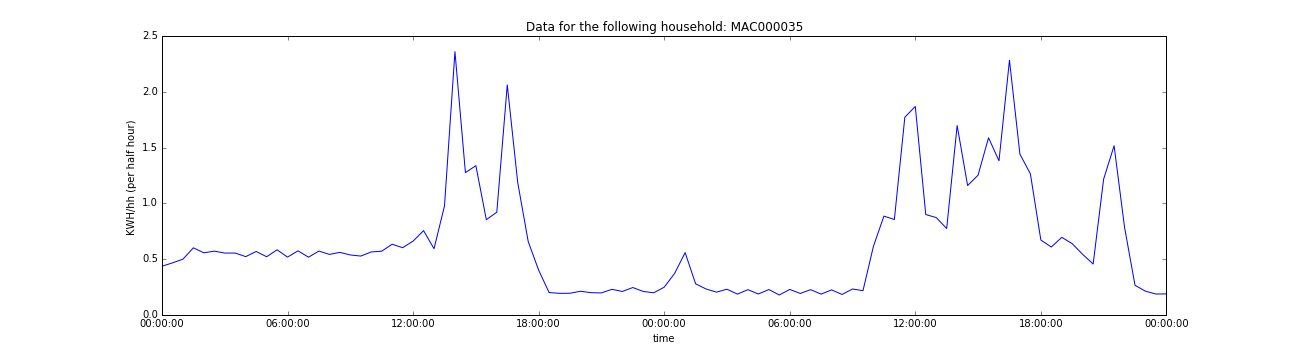
\includegraphics[height=1.5in, width=\textwidth]{../img/fig1.png}

   \caption{Two days energy demand for a typical household.}

    \label{fig:MAC000035_2days_sample}
    \end{center}
\end{figure}

\end{frame}


\section{Model}
%3
\begin{frame}
\frametitle{Modeling Technique}
I have developed complex model which consists of a number of ARMA sub-models. Below is outline of its architecture:
\\
\begin{itemize}
\item I split day into a several time intervals and train a separate sub-model for each time interval over a number of days of previous data.
\item Each sub-model produces a single prediction for one day ahead of training data such that all sub-models together produce forecast for entire day.
\item Smart meter data present 48 records for a single day with half hour interval. Thus, the entire model is a combination of 48 sub-models trained separately for each time interval.
\end{itemize}
\end{frame}

%4
\begin{frame}
\frametitle{Performance of the Model}
Each model can be trained on weekdays/weekends subsets of data only as well as on data with no split with respect to different parts of week.
\begin{figure}[htb]
\begin{center}
    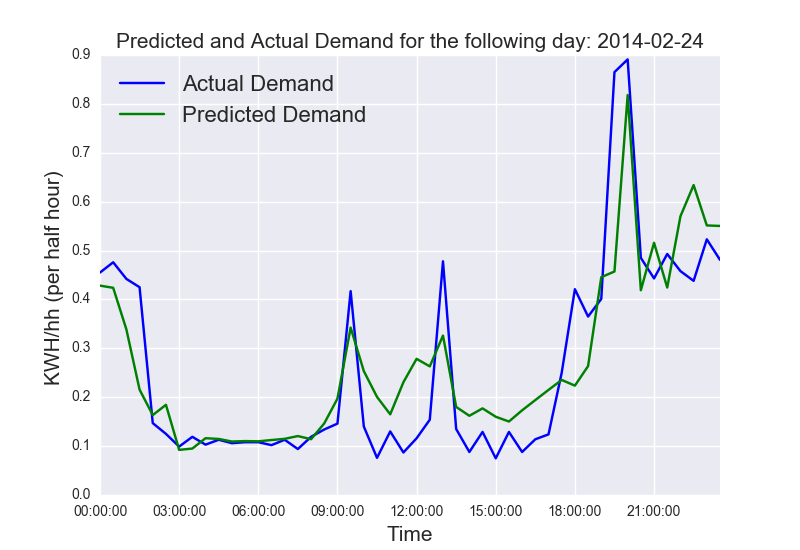
\includegraphics[height=1.6in, width=0.9\textwidth]{../img/fig2a.png}

    \caption{Weekdays 48 sub-models model forecast for one day. The model was trained on 350 days.}

    \label{fig:MAC000002_Model48weekdays}
    \end{center}
\end{figure}

\end{frame}

\begin{frame}

\begin{figure}[htb]
\centering
 \begin{tabular}{@{}cc@{}}
   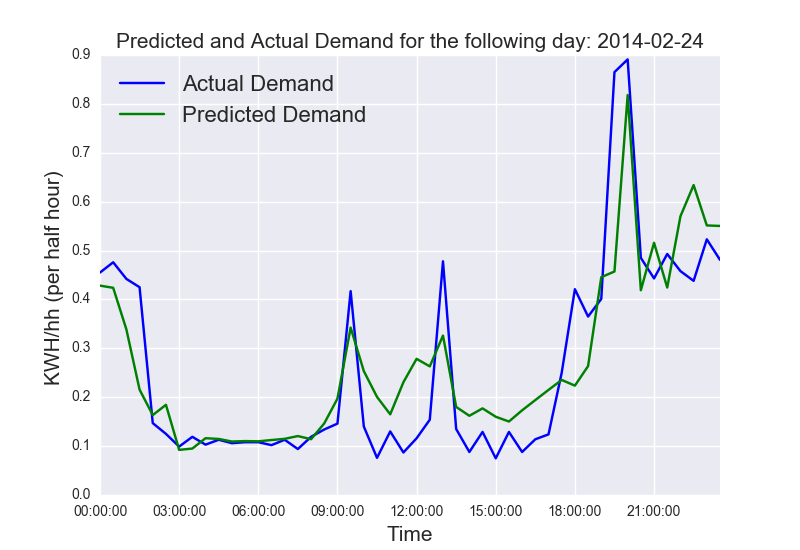
\includegraphics[width=.5\textwidth]{../img/fig2a.png} &
   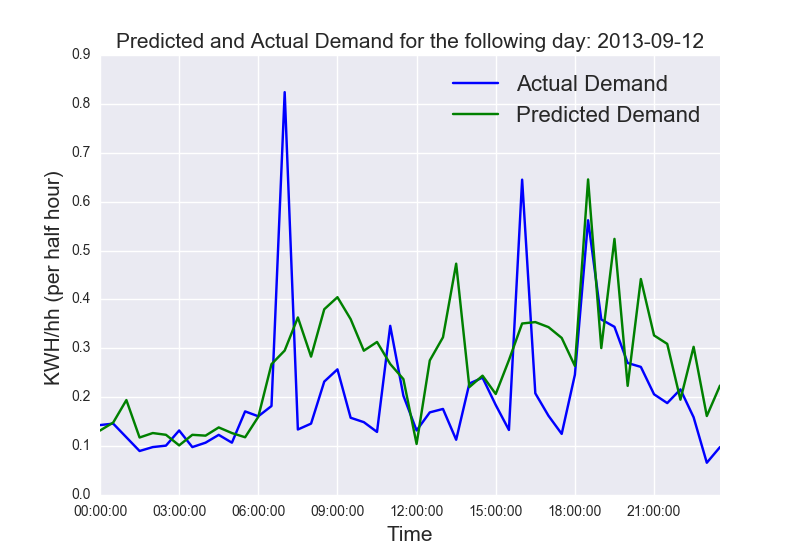
\includegraphics[width=.5\textwidth]{../img/fig2b.png}   \\
   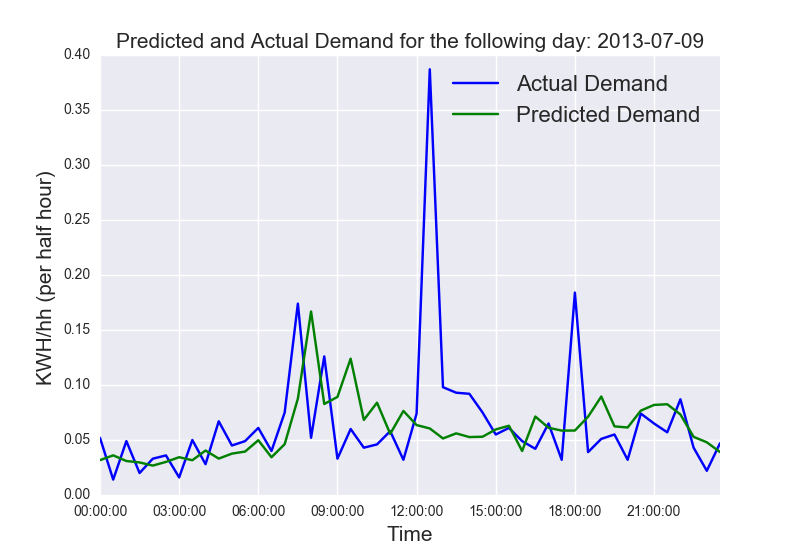
\includegraphics[width=.5\textwidth]{../img/fig2c.png} &
   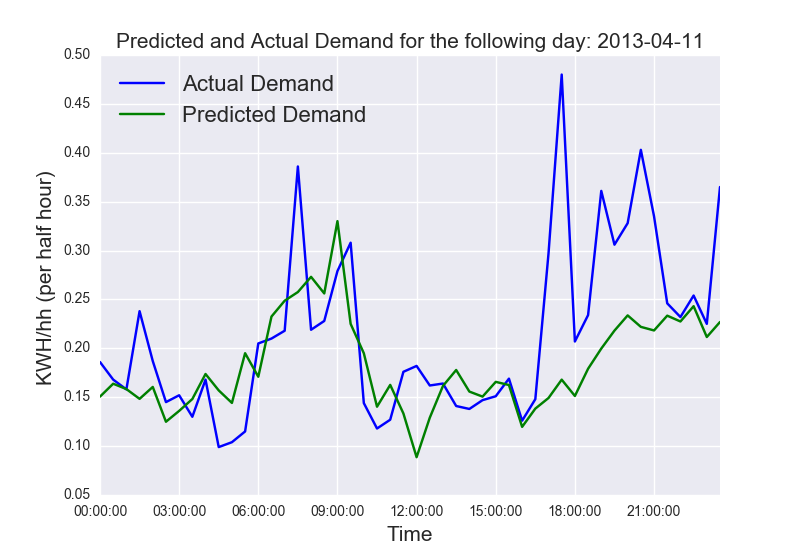
\includegraphics[width=.5\textwidth]{../img/fig2d.png}
  \end{tabular}
  \caption{Weekdays model forecast for one day for 4 households.}
\end{figure}


\end{frame}


\section{Results}
%5
\begin{frame}
\frametitle{Predictions of the Battery Charge-Standby-Discharge Cycles}

\begin{figure}[htb]
\centering
 \begin{tabular}{@{}cc@{}}
   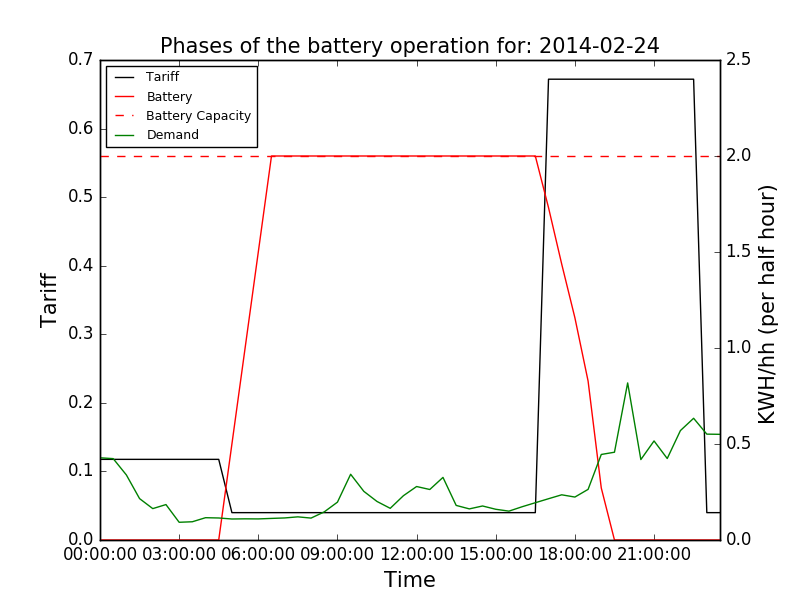
\includegraphics[width=.43\textwidth]{../img/fig3a.png} &
   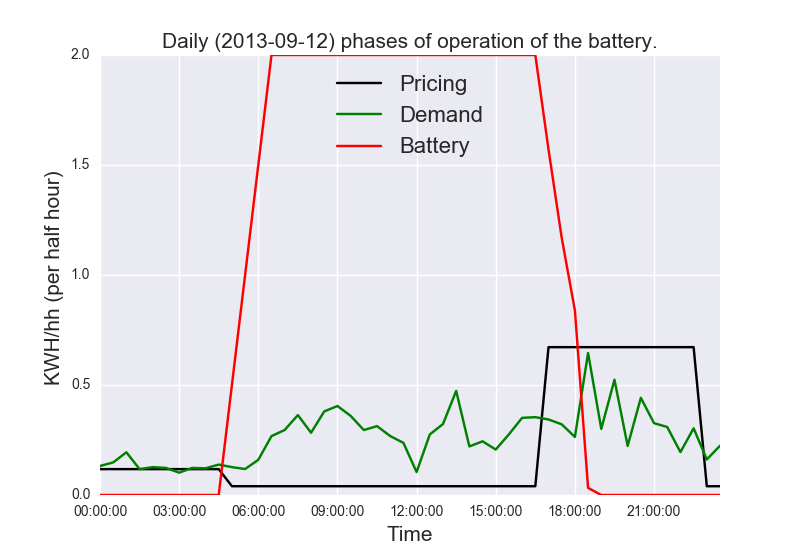
\includegraphics[width=.43\textwidth]{../img/fig3b.png}   \\
   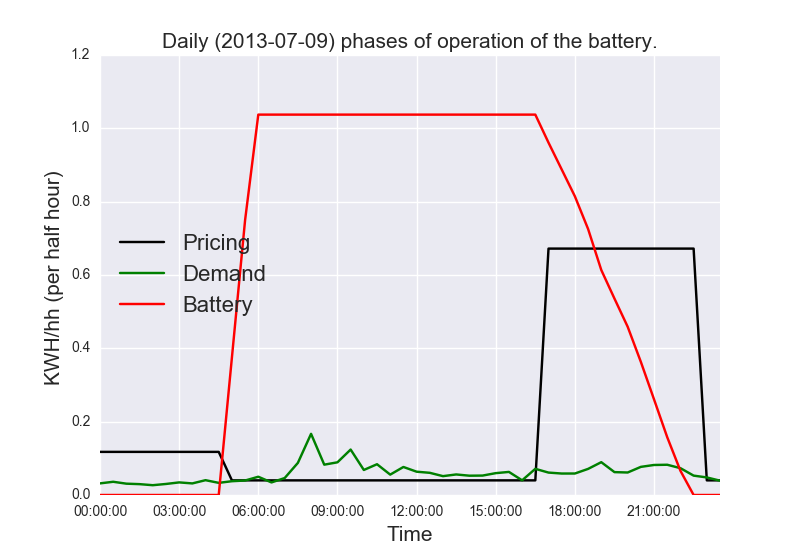
\includegraphics[width=.43\textwidth]{../img/fig3c.png} &
   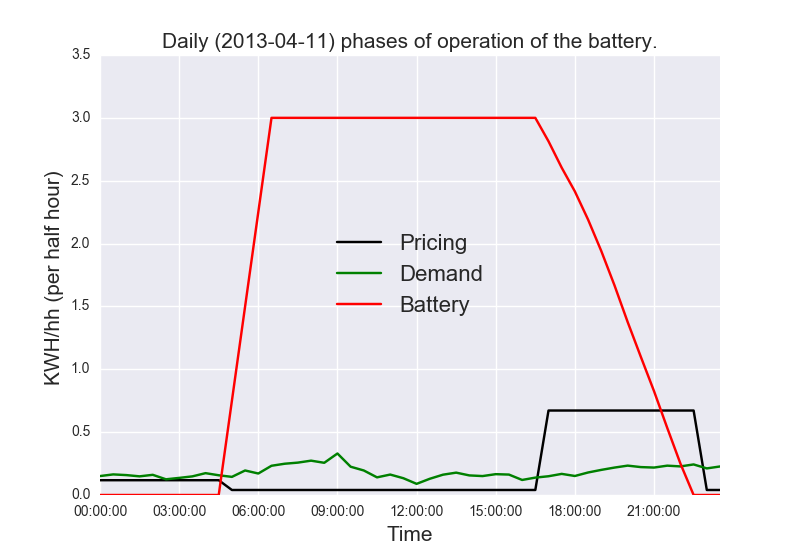
\includegraphics[width=.43\textwidth]{../img/fig3d.png}
  \end{tabular}
  \caption{Weekdays forecast for the battery cycles for 4 households.}
\end{figure}

\end{frame}

%6
\begin{frame}
\frametitle{Ruler to Determine Optimal Size of Battery}

\begin{figure}[htb]
\begin{center}
    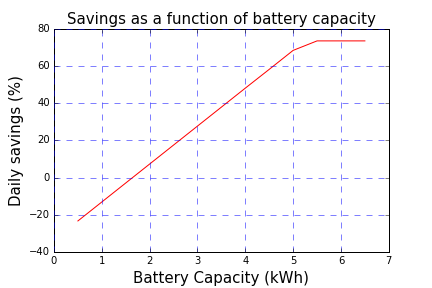
\includegraphics[height=1.6in, width=0.9\textwidth]{../img/fig4.png}

    \caption{Forecast of potential savings for a particular household and various battery capacities.}

    \label{fig:fig4}
    \end{center}
\end{figure}


\end{frame}


\section{The End}
%7
\begin{frame}

\begin{center}

\textbf{\LARGE Thank You!}\\

\end{center}

$\bullet$ GitHub: \url{https://github.com/AnatolyPavlov}\\

$\bullet$ LinkedIn: \url{https://www.linkedin.com/in/anatolypavlov}\\

$\bullet$ Email: pavlovanatoly2012@gmail.com

\end{frame}


\end{document}